We set up our optimization with two different turbine groups. We assigned each turbine to one of two groups, where all turbines in a group had the same tower hub height, rotor diameter, turbine rating, tower diameter, and tower shell thickness. Manufacturing each tower with custom dimensions may be very expensive, and further study will be necessary to determine if it is worth the additional cost and complexity to design each turbine individually. We chose two groups because our previous study in which we optimized wind farms with different turbine heights indicated that the most benefit comes from increasing from one height group to two. Any benefit from introducing more groups was marginal\cite{stanley2018}. We parameterized the tower by specifying the diameter and shell thickness at the bottom, midpoint, and top of the tower and then linearly interpolating diameter and shell thickness at points in between. 
        
        It may be beneficial to do a binary optimization in which each turbine can change the turbine group to which it belongs, but this greatly increases the complexity of the optimization and makes it gradient-free. Binary variables, such as turbine group assignment, have no intermediate values. They are either one or the other. This means there is no way to use gradients in their optimization. Gradient-free optimization is more computationally expensive, which severely limits the number of design variables we can include in the problem. To maintain the gradient-based optimization, we assigned each turbine to one of the groups before starting the optimization. Once assigned a turbine could not switch to the other group. In this study, we only examine an equal weighting of turbines in each group, but additional benefit may come from optimally choosing the number of turbines in each group.% However, we did explore the effect of including different ratios of the different turbine groups, including 1-1, 2-1, and 3-1.
        
        We ran several cases in which different design variables were included in the problem to allow comparison of their effects on COE. In all, the design variables we included were the position of each turbine ($x_i,y_i$), the tower height of each group ($H_1, H_2$), the rotor diameter of each group ($D_1, D_2$), the rated power of each group ($R_1, R_2$), the tower diameter of each group ($d_{1,j}, d_{2,j}$), and the tower shell thickness of each group ($t_{1,j}, t_{2,j}$). Index j refers location on the tower (j=1 is at the bottom, j=2 at the midpoint, j=3 at the top), meaning there are six total variables to define diameter (three for each height group), and six to define the tower shell thickness.
                
        The position of each turbine was constrained so that it could not be within two rotor diameters of any other turbine in the wind farm. Because rotor diameter was a design variable, this constraint was defined such that the distance between any two turbines in the wind farm was greater than the sum of the two rotor diameters. Also, for the Princess Amalia layouts, each turbine was constrained so that it could not leave the convex hull of the original turbine layout at the beginning of the optimization. For the circular farm, there was a circular wind farm boundary defined by the radius from the baseline turbine layout. %This constraint ensured that the turbines did not simply spread far apart to decrease COE. 
        The tower heights and rotor diameters were also constrained such that the tower height would be taller than the rotor radius plus a ground clearance, which we set as 10 m. This allowed us to separate the heights of different turbines while keeping a safe distance from the ground. 
        Both the rotor diameter and the turbine rating were constrained by the lowest and highest values that were included in the RotorSE optimization. This constraint is defined from the upper and lower functioning limits of RotorSE. The lower limits were never active in these optimizations, however some of the upper limits were active as will be seen in the Results section.
        %but is only a formality as it was never active in any of the optimization runs we did. 
        The tower diameter was constrained to be less than 6.3 m for transportation, and greater than or equal to 3.6 at the top, to allow for the connection to the nacelle. Each tower was also structurally constrained by the shell buckling and natural frequency of the tower. The shell buckling constraint was applied to each height group for both the maximum thrust conditions and the survival load, with a safety factor of 1.35 for the loads and 1.1 for buckling resistance. The first natural frequency of the tower was constrained to be greater than the frequency at which the blades rotate and less than the blade passing frequency, with a factor of safety of 1.1. The diameter-to-thickness ratio was constrained to be greater than 120 at any point, to allow for welding. The optimization can be expressed:
        
        \begin{equation}
			\begin{aligned}
				& \text{minimize}
					& & \text{COE} \\
                & \text{w.r.t.} 
                	&& x_i,~ y_i,~ H_{1,2},~ D_{1,2},~ R_{1,2},~ d_{(1,j)},~ d_{(2,j)},~ t_{(1,j)},~t_{(2,j)}\\
                		&&& i = 1, \ldots, n; \; j = 1,~2,~3 \\
				& \text{subject to}
% 					& & x_{\text{initial, min}} \leq x_i \leq x_{\text{initial, max}} \\
					& & \text{boundary constraints} \\
%                         &&& y_{\text{initial, min}} \leq y_i \leq y_{\text{initial, max}} \\
						&&& \sqrt{(x-x_i)^2+(y-y_i)^2} \geq 2D_{\text{rotor}} \\
						&&& H_1-\frac{D_1}{2}, H_2-\frac{D_2}{2} \geq 10~ \text{m}\\
                		&&& d_{(1,j),(2,j)} \leq 6.3~ \text{m}\\
                		&&& d_{(1,top),(2,top)} \geq 3.6~ \text{m}\\
						&&& \frac{3\hspace{0.08cm}\Omega}{1.1} \geq f_{1,2} \geq 1.1\hspace{0.08cm}\Omega \\
                		&&& \text{shell buckling margins: max thrust} \leq 1 \\
                        &&& \text{shell buckling margins: survival load} \leq 1 \\
                		&&& \frac{d_{(1,j)}}{t_{(1,j)}},\frac{d_{(2,j)}}{t_{(2,j)}} \geq 120\\
                        &&& 46~ \text{m} < D_1,D_2 < 160~ \text{m}  \\
                        &&& 500~ \text{kW} < R_1,R_2 < 10,000~ \text{kW} \\
			\end{aligned}
		\end{equation}
%
Note that i is the index defining the wind turbine, and j is the index describing the location on the tower.
        
        The gradients for this optimization were all analytic. We calculated the partial derivatives of each small section of the model and included each part in a framework called OpenMDAO \cite{gray2010openmdao}, which calculates the gradients of the entire system. The analytic gradients are significant because they are more accurate, converging to better solutions, and converge on the solution much faster that finite difference gradients. More importantly, they allow us to solve much larger optimization problems. % These analytic gradients allow coupled optimization of turbine position, height, diameter and thickness, and yaw in each wind direction. Including yaw introduces thousands of design variables, and is nearly impossible to optimize with gradient-free methods and very time-consuming with finite difference gradients.  
        
We optimized two different wind farms, each with different wind shear exponents and turbine spacing multipliers as will be explained later in this section. The first wind farm is the Princess Amalia wind farm layout which has 60 wind turbines, and which was optimized with the Princess Amalia wind data shown in Figures \ref{amalia} and \ref{amalia_speeds}. The farm boundary for this wind farm is the convex hull of the original Princess Amalia wind farm. The baseline turbine layout and boundaries are shown in Figure \ref{amalia_layout}. The turbines in the Princess Amalia wind farm are Vestas 2 Megawatt wind turbines, which have a rotor diameter of 80 meters. Therefore, we used a baseline rotor diameter of 80 meters and a baseline power rating of 2 Megawatts. The baseline hub height used in this study was 100 meters. The second wind farm is a fictional 32 turbine wind farm with a circular boundary. The baseline layout and boundary is shown in Figure \ref{circular_layout}. This wind farm was optimized with the Alturas wind data shown in Figure \ref{alturas}. The baseline rotor diameter, power rating, and hub height for this farm are the same as for the Princess Amalia wind farm. 

\begin{figure}[htbp]
  \centering
  \subfloat[\label{circular_layout}Circular wind farm layout.]{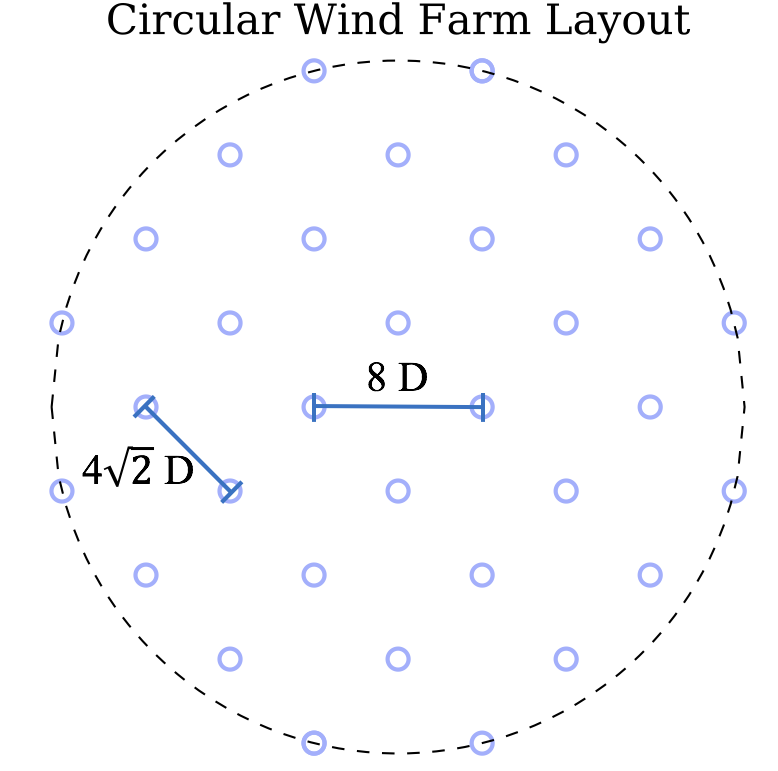
\includegraphics[width=0.4\textwidth]{Figures/circular.png}}
  \subfloat[\label{amalia_layout}Princess Amalia wind farm layout.]{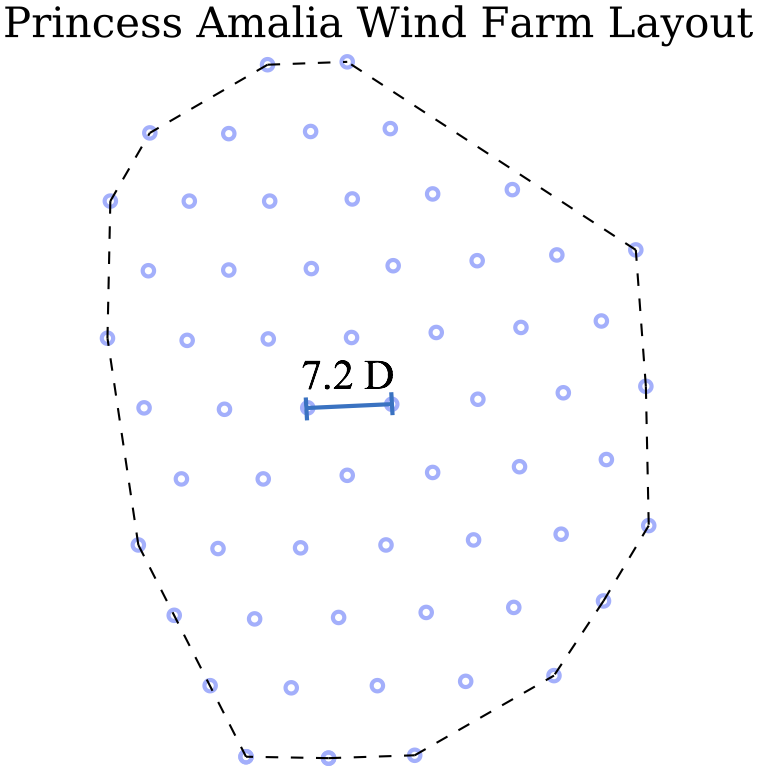
\includegraphics[width=0.4\textwidth]{Figures/amalia.png}}
  \caption{\label{layouts} The two different wind farm designs that were optimized. On the left is a contrived circular wind farm design with 32 turbines. On the right is the Princess Amalia wind farm, an offset grid design with 60 wind turbines. }
\end{figure}

We optimized each of the wind farms shown in Figure \ref{layouts} with three different wind shear exponents (0.075, 0.175, 0.275), and three different spacing multipliers (0.5, 1.0, 1.5). The wind shear exponent defines how fast the wind speed changes with height, as seen in Equation \ref{Eq:shear}. Low shear exponents are typical over open water or flat plains, while higher shear exponents exist in areas with a lot of large trees or buildings. Figure \ref{shear_profile} shows the wind speed profiles of the three shear exponents we used. For a shear exponent of 0.075, there is only an 8.6\% increase in the wind speed from the reference height of 50 meters to 150 meters. For a shear exponent of 0.175 there is a wind speed increase of 21.2\% for the same height difference, and for a shear exponent of 0.275 the wind speed increase is 35.3\% from 50 to 150 meters. We also optimized each wind farm for different turbine spacings by adjusting the turbine locations by some spacing multiplier, $\beta$.  This is simply some constant multiplied to each turbine location. The wind farm boundaries were adjusted accordingly with the spacing multipliers. Figures \ref{amalia_spacings} and \ref{circle_spacings} show both of the wind farms adjusted by the spacing multipliers.


\begin{figure}[htbp]
  \centering
  \subfloat[]{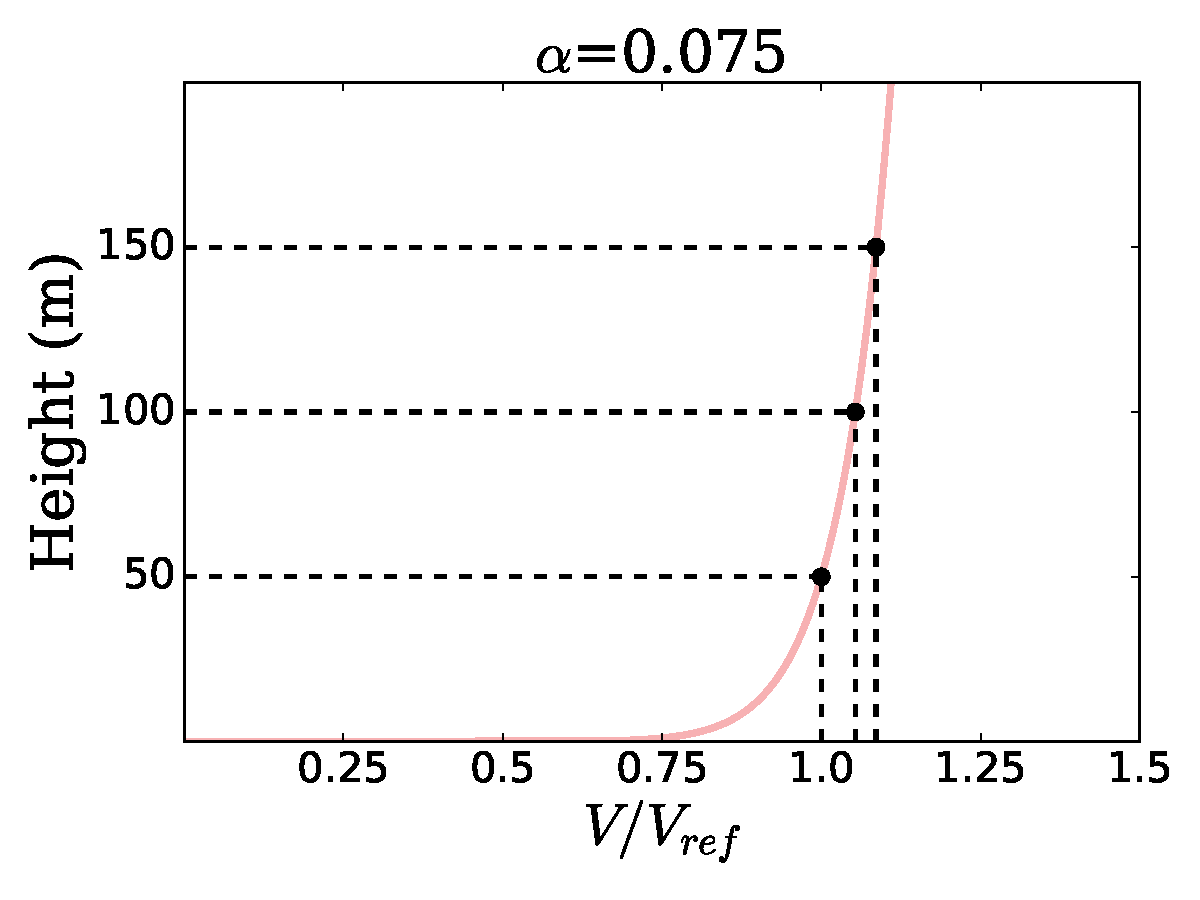
\includegraphics[width=0.5\textwidth]{Figures/windProfile_0_075.pdf}\label{wp075}}\\
  \subfloat[]{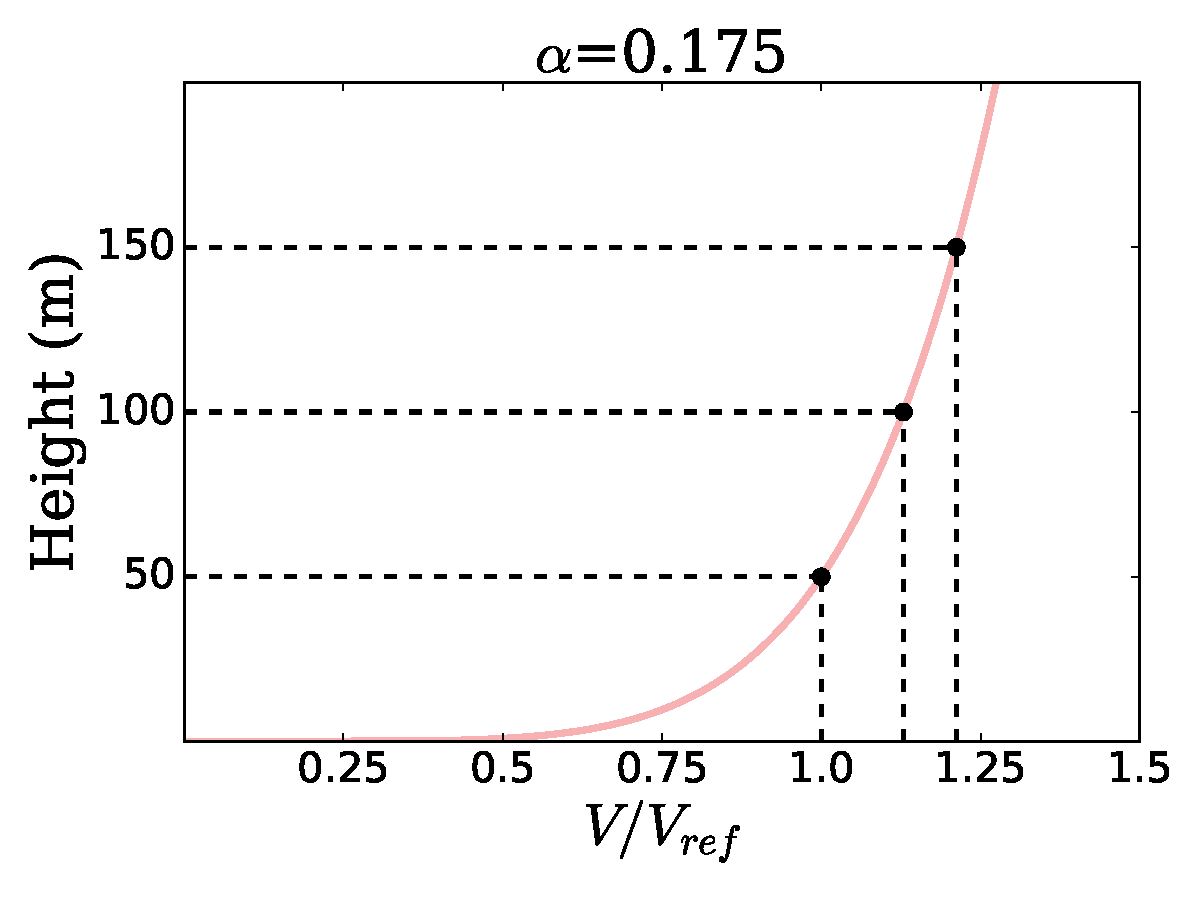
\includegraphics[width=0.5\textwidth]{Figures/windProfile_0_175.pdf}\label{wp175}}\\
  \subfloat[]{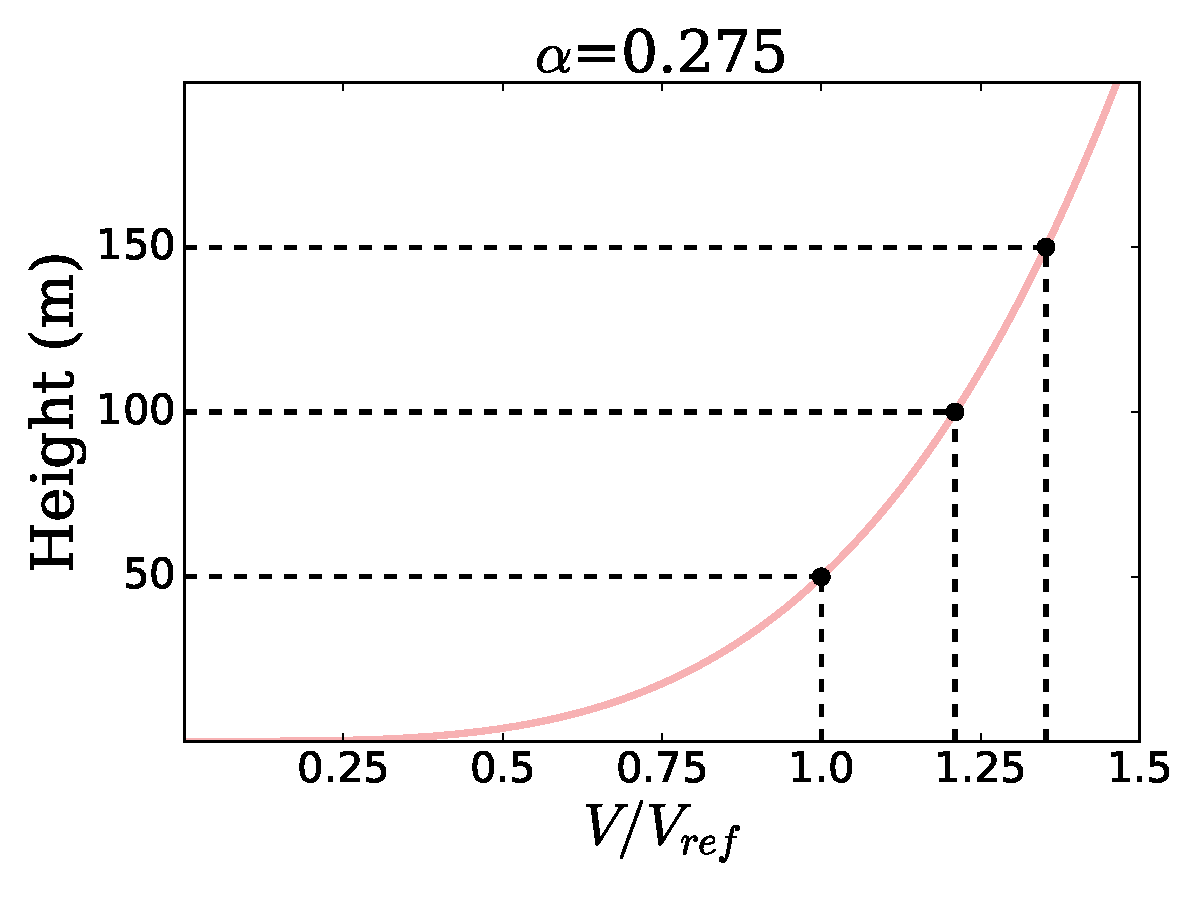
\includegraphics[width=0.5\textwidth]{Figures/windProfile_0_275.pdf}\label{wp275}}
  \caption{\label{shear_profile}The wind speed profiles for various wind shear exponents. With lower shear exponents, like $\alpha=0.075$ shown in Figure \ref{wp075}, the wind speed does not vary dramatically with height. For higher wind shear, like $\alpha=0.275$ shown in Figure \ref{wp275}, there is a significant wind speed increase with height.}
\end{figure}

\begin{figure}[htbp]
  \centering
  \subfloat[]{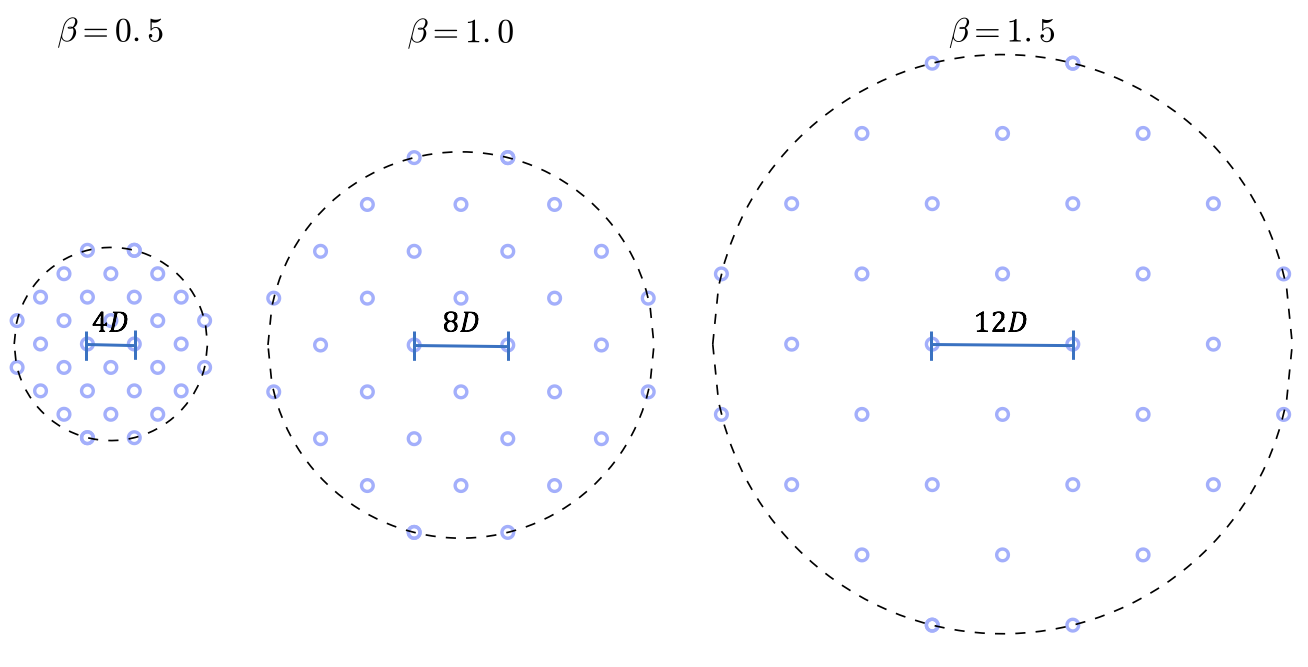
\includegraphics[width=\textwidth]{Figures/circle_spacings.png}\label{circle_spacings}}\\
  \subfloat[]{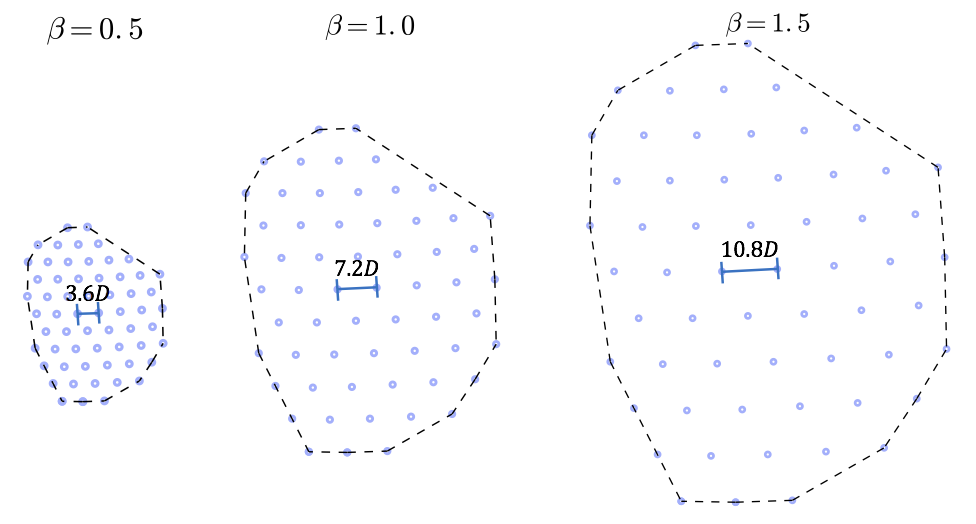
\includegraphics[width=\textwidth]{Figures/amalia_spacings.png}\label{amalia_spacings}}  
  \caption{\label{farm_spacings}The six wind farm layouts optimized in this study. The same two layouts were multiplied by a spacing multiplier, $\beta=0.5,1.0,1.5$, which changed the wind farm size and the averaging spacing between wind turbines. }
\end{figure}

The results of gradient-based optimization, especially for problems with many local minima, are sensitive to the starting location. As in most optimization problems, there is no guarantee that the solution is the global solution. The best results can be achieved with a multiple-start approach, where several different starting points are used for each condition, and the best solution is used. In our study, we started each turbine location from the Princess Amalia or circular wind farm baseline locations in Figures \ref{amalia_spacings} and \ref{circle_spacings}, each perturbed by a random amount. All of the other design variables were initialized randomly.

% \begin{figure}[htbp]
%   \centering
%   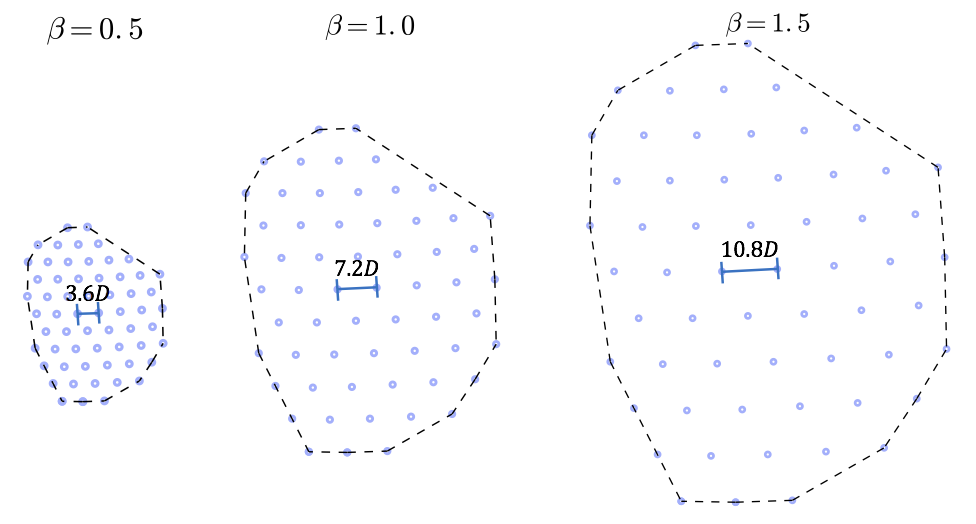
\includegraphics[width=\textwidth]{Figures/amalia_spacings.png}
%   \caption{\label{amalia_spacings} \textbf{CAPTION HERE}}
% \end{figure}

% \begin{figure}[htbp]
%   \centering
%   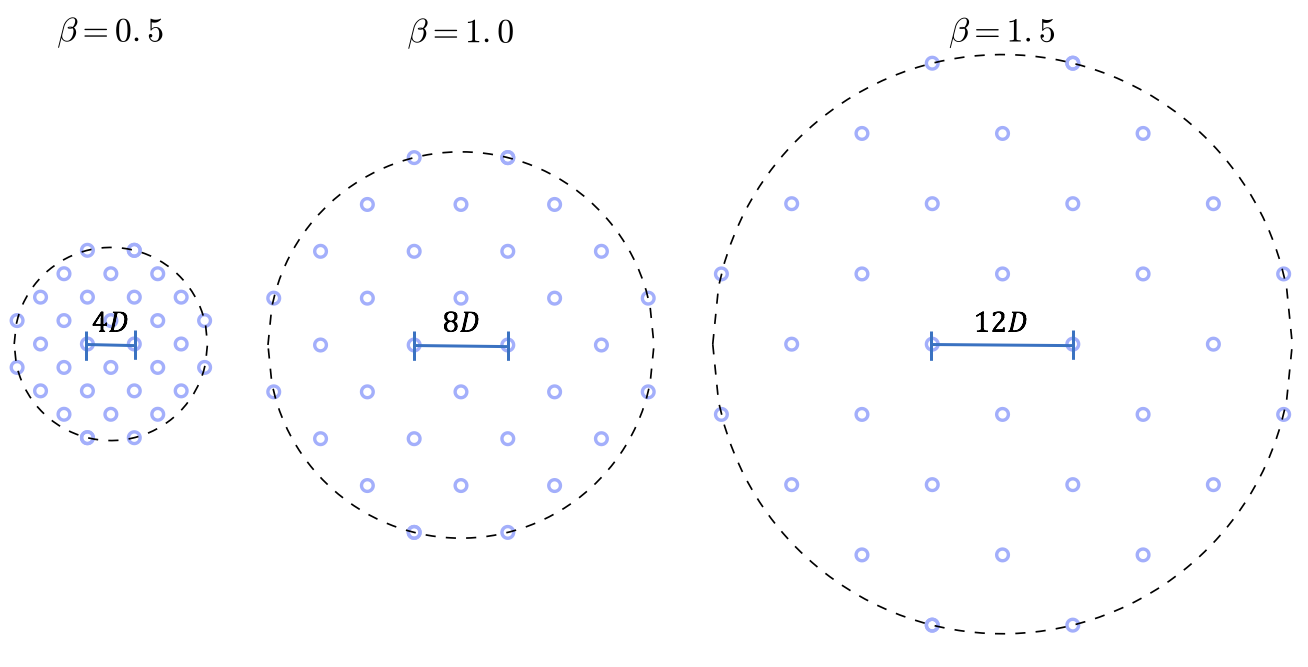
\includegraphics[width=\textwidth]{Figures/circle_spacings.png}
%   \caption{\label{circle_spacings} \textbf{CAPTION HERE}}
% \end{figure}


% \begin{figure}[htbp]
%   \centering
%   \subfloat[]{\includegraphics[trim={0 0 0 0},clip,width=0.33\textwidth]{Figures/amalia0_5.pdf}\label{wp075}}
%   \subfloat[]{\includegraphics[trim={0 0 0 0},clip,width=0.33\textwidth]{Figures/amalia1_0.pdf}\label{wp175}}
%   \subfloat[]{\includegraphics[trim={0 0 0 0},clip,width=0.33\textwidth]{Figures/amalia1_5.pdf}\label{wp275}}
%   \caption{\label{shear_profile}\textbf{CAPTION HERE}}
% \end{figure}